\section{Component Diagram}
Nella figura \ref{fig:ComponentDiagram_iterazione3} è riportato il diagramma a componenti dell'applicazione dove sono state evidenziate le interfacce e i componenti inseriti nell'iterazione 3. 
\begin{figure}[h!]
	\centering
	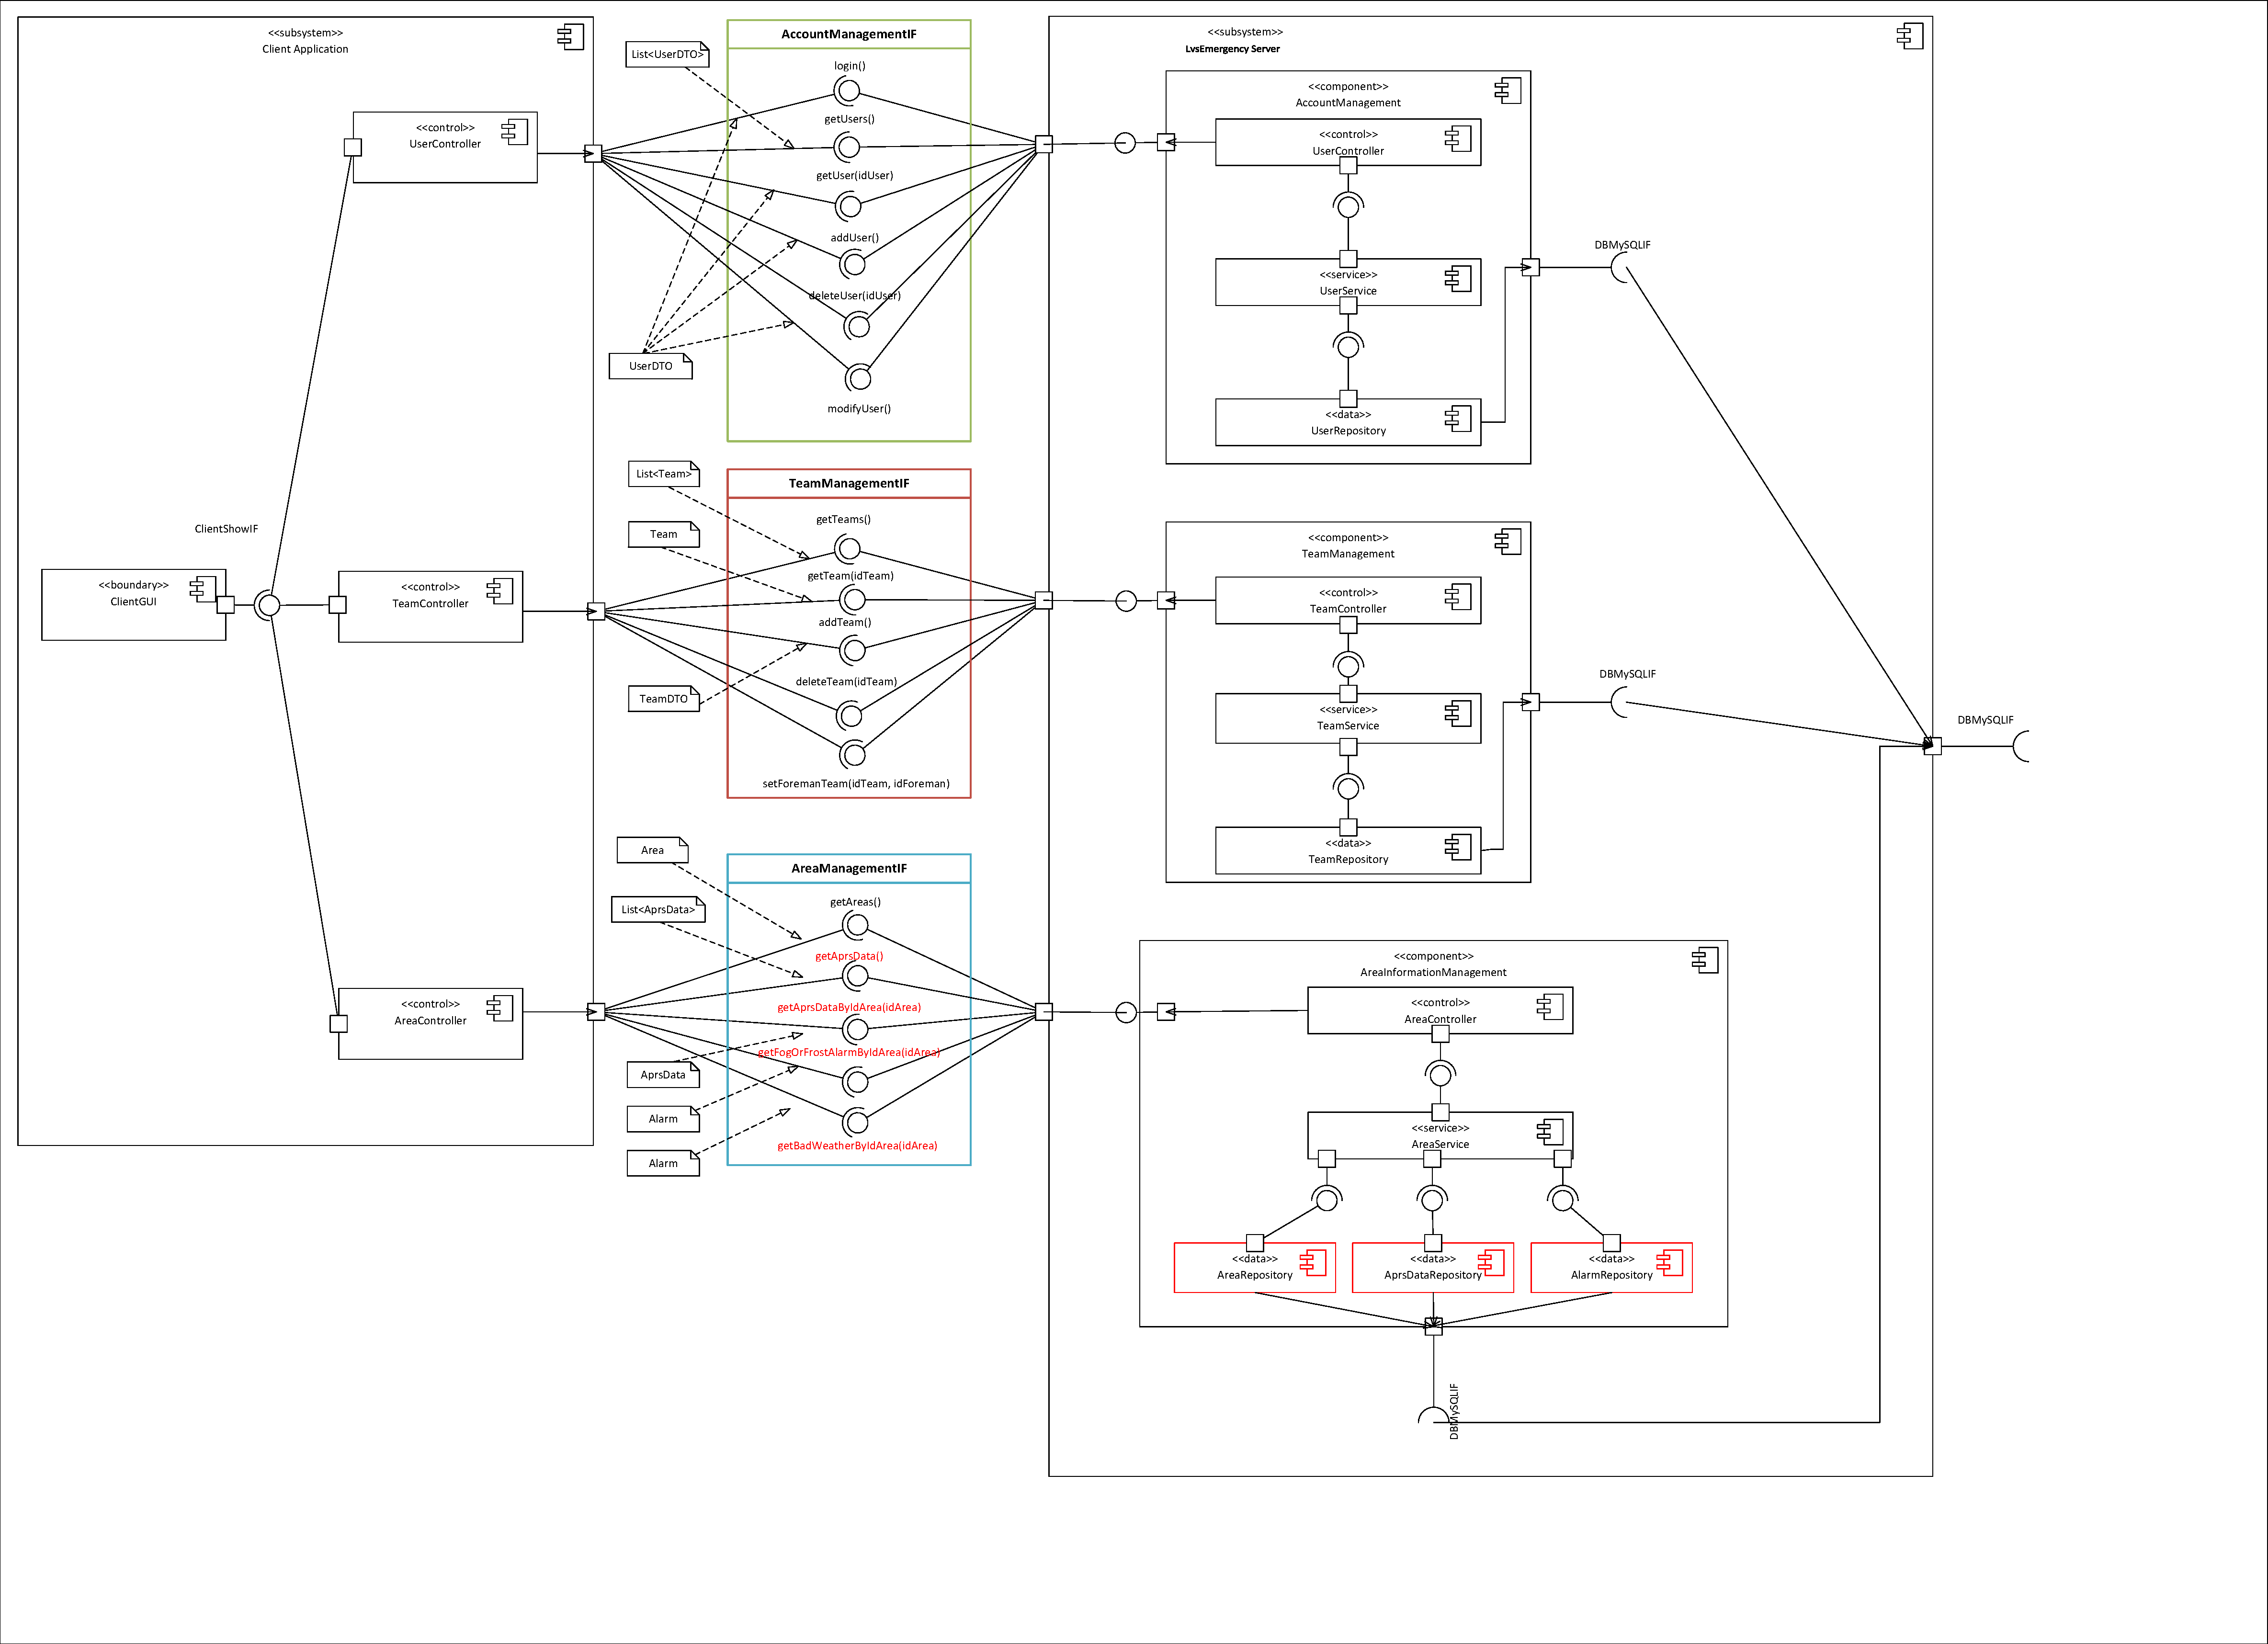
\includegraphics[width=1\linewidth]{./Iterazione 3/OtherFiles/UML - Component view}
	\caption{Component Diagram.}
	\label{fig:ComponentDiagram_iterazione3}
\end{figure}

\clearpage

\section{Class Diagram}
Di seguito è riportata la specifica della struttura dati \texttt{PositionDTO}(\Fig\ref{fig:ClassDiagramDTO_iterazione3}). Questo struttura dati è particolarmente utile per incapsulare in un unico oggetto sia le informazioni della posizione che il nome ed il cognome dell'utente a cui appartiene la posizione.

\begin{figure}[h!]
	\centering
	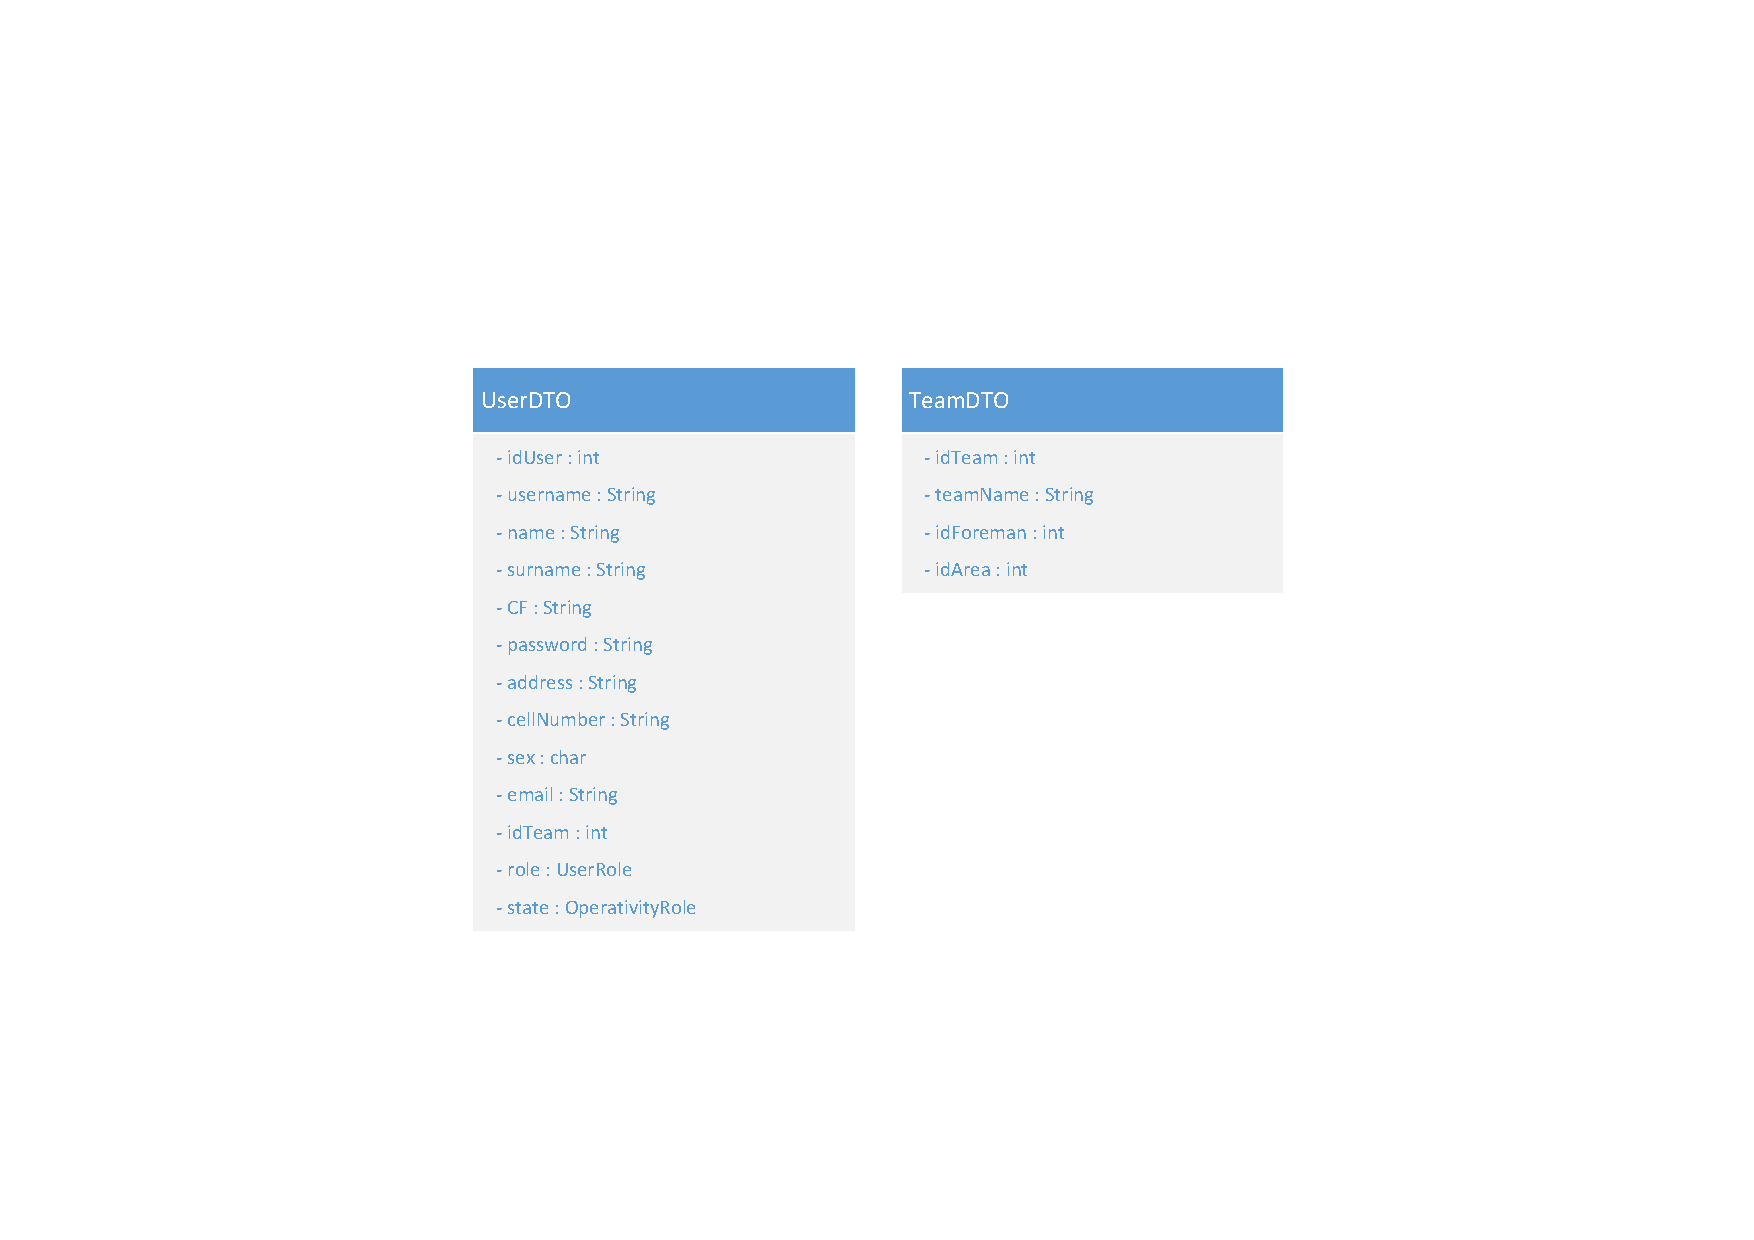
\includegraphics[width=0.7\linewidth]{./Iterazione 3/OtherFiles/DTOSpecification}
	\caption{Class Diagram \texttt{PositionDTO}.}
	\label{fig:ClassDiagramDTO_iterazione3}
\end{figure}

\clearpage

\section{Interface and Package Diagram}
Le API per ricevere i dati meteorologici e gli allarmi sono state implementate nel package \textit{AreaInformationManagement} (\Fig\ref{fig:InterfaceDiagram_iterazione3}) e sono gestite dal controller \texttt{AreaController}. I package \textit{alarm} e \textit{data} sono stati riportati per completezza: al loro interno sono state inserite le classi che gestiscono rispettivamente gli allarmi e i dati provenienti dalle stazioni APRS. Invece, le API che si occupano dell'ottenimento dell'ultima posizione disponibile di un utente attivo e dell'invio della nuova posizione di un utente sono state implementate nel package \textit{AccountManagment}

\begin{figure}[h!]
	\centering
	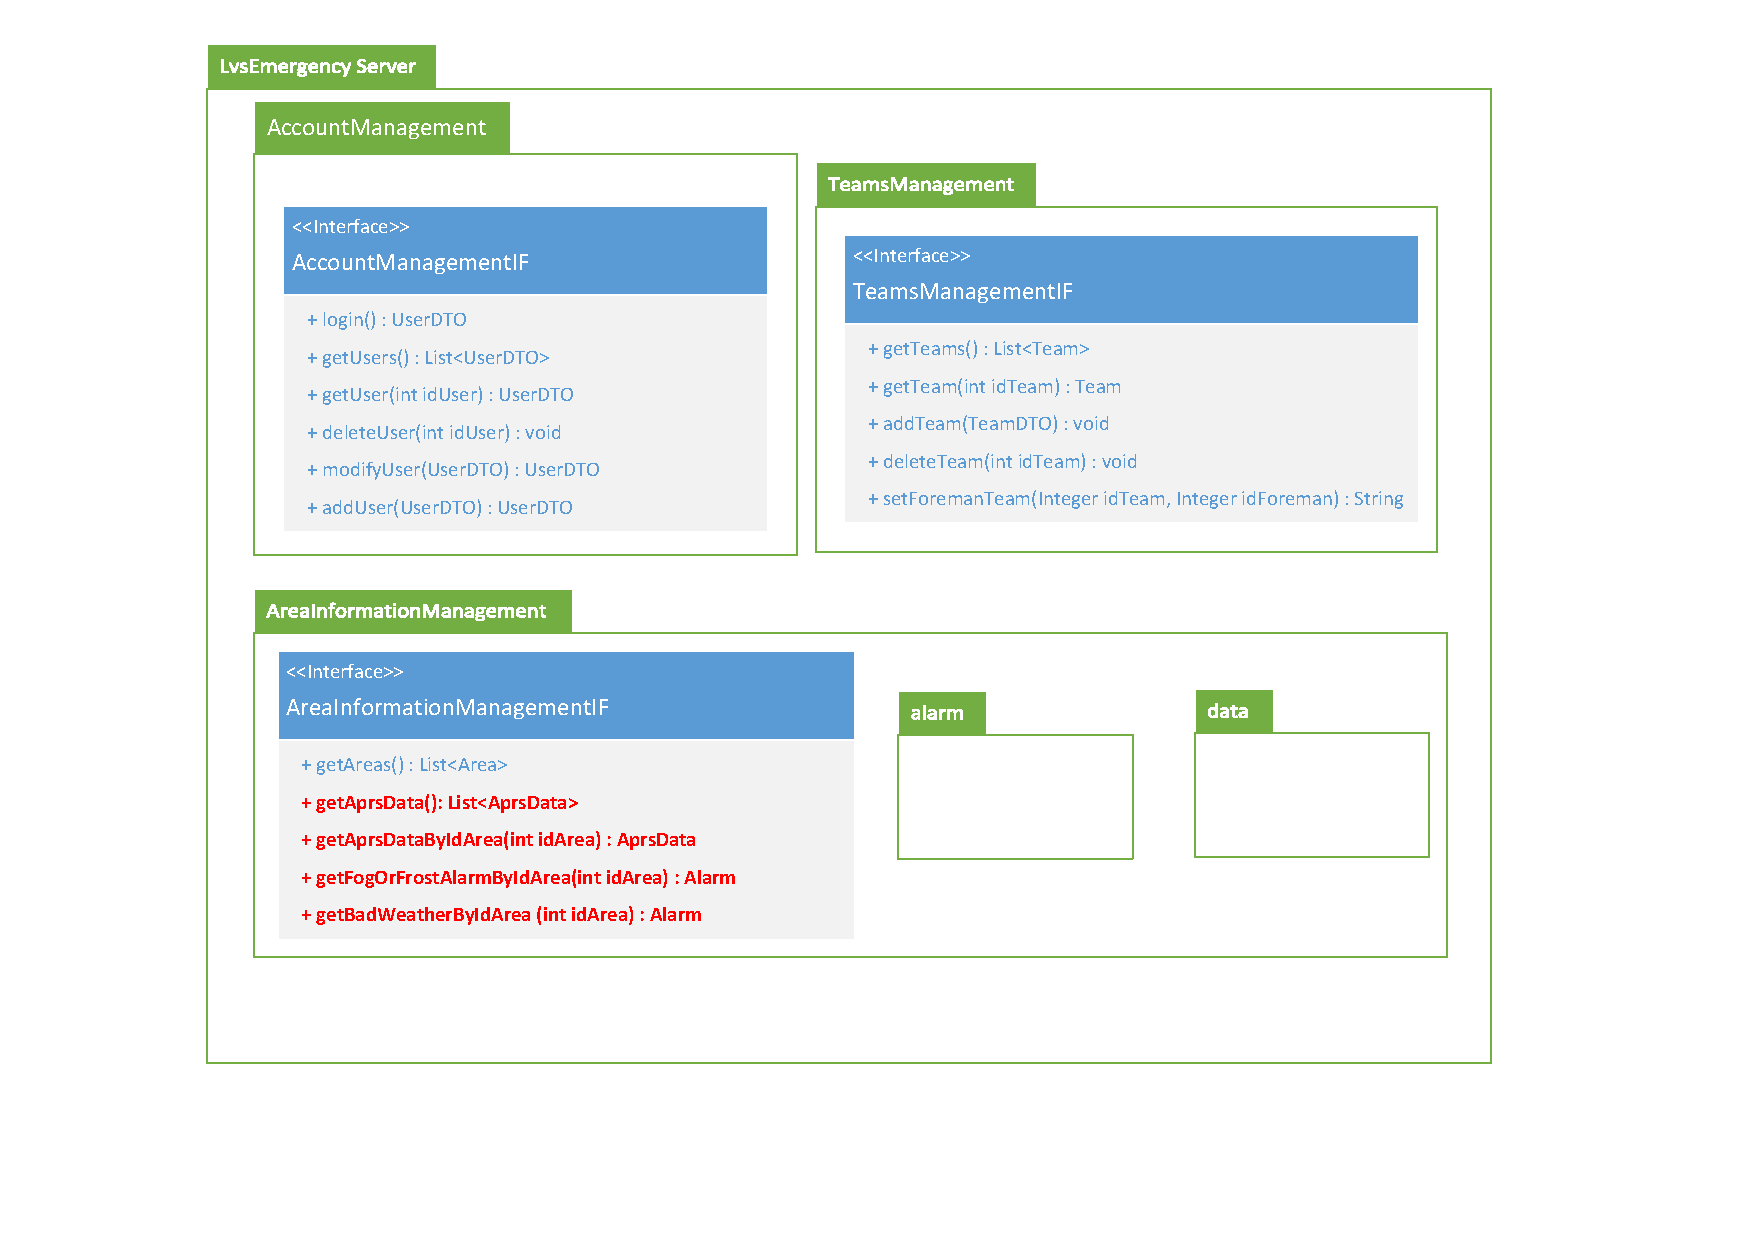
\includegraphics[width=0.8\linewidth]{./Iterazione 3/OtherFiles/UML - Interface Diagram}
	\caption{Interface and Package Diagram.}
\label{fig:InterfaceDiagram_iterazione3}
\end{figure}